\chapter{Treffen am 15.12.2014}
\section{Anwesende Personen}
\begin{itemize}
	\item Stefan Biereigel
	\item Rene Winkler
	\item Mathias Fugmann
	\item Junlong Yin
\end{itemize}

\section{Besprochen bzw. Bearbeitet}
Vor dem Abschluss der Arbeit an der Entscheidungsmatrix wurde noch einmal unverfänglich über die verschiedenen Konzepte diskutiert und sich über mögliche Unzulänglichkeiten Gedanken gemacht. 

Außerdem kamen die folgenden Punkte im Verlauf des Gesprächs auf, die eventuell im finalen Design noch berücksichtigt werden sollten:
\begin{itemize}
	\item Bedienung mit mehreren Schnittstellen (Joystick, Tasten, ...) sollte möglich sein $\rightarrow$ es muss eine Hierarchie definiert werden.
	\item Mehrere Bedienmöglichkeiten erweitern die Anzeigemöglichkeiten auf dem Display enorm (künstlicher Horziont als Beispiel) - sie können (und müssen) auf das verwendete Eingabegerät angepasst werden
	\item Ein Beschleunigungssensor sollte abschaltbar sein, um keine Probleme beim Weglegen der Fernbedienung zur verursachen.
	\item Es könnte einen Schiebeschalter zur Deaktivierung dieses Sensors geben, der dann auch gleich die Fernbedienung ausschalten könnte (3 Stellungen: Aus, Ein, Ein mit Beschleunigungssensor)
\end{itemize}

Die Arbeit wird sich am Ende auf drei Hauptaufgabenbereiche aufteilen (Software, Hardware, Mechanik), alle haben ungefähr gleichen Umfang und Wichtigkeit, wobei Software noch den größten Unsicherheitsfaktor darstellt.

Rene Winkler tauschte mit Prof. Voß die Kontaktdaten zum FB SciTec aus, sodass eine Voranfrage zur Nutzungsmöglichkeit eines 3D-Druckers stattfinden kann. Abgeklärt werden muss dafür außerdem noch, welche Dateiformate notwendig sind, ob weitere technische Zeichnung für die Fertigung gebraucht werden und wie entstehende Kosten beglichen werden können.

Es wurde eine Skizze für ein mögliches Aussehen der Fernbedienung angefertigt, die im folgenden zu sehen ist.

\begin{figure}[h]
	\centering
	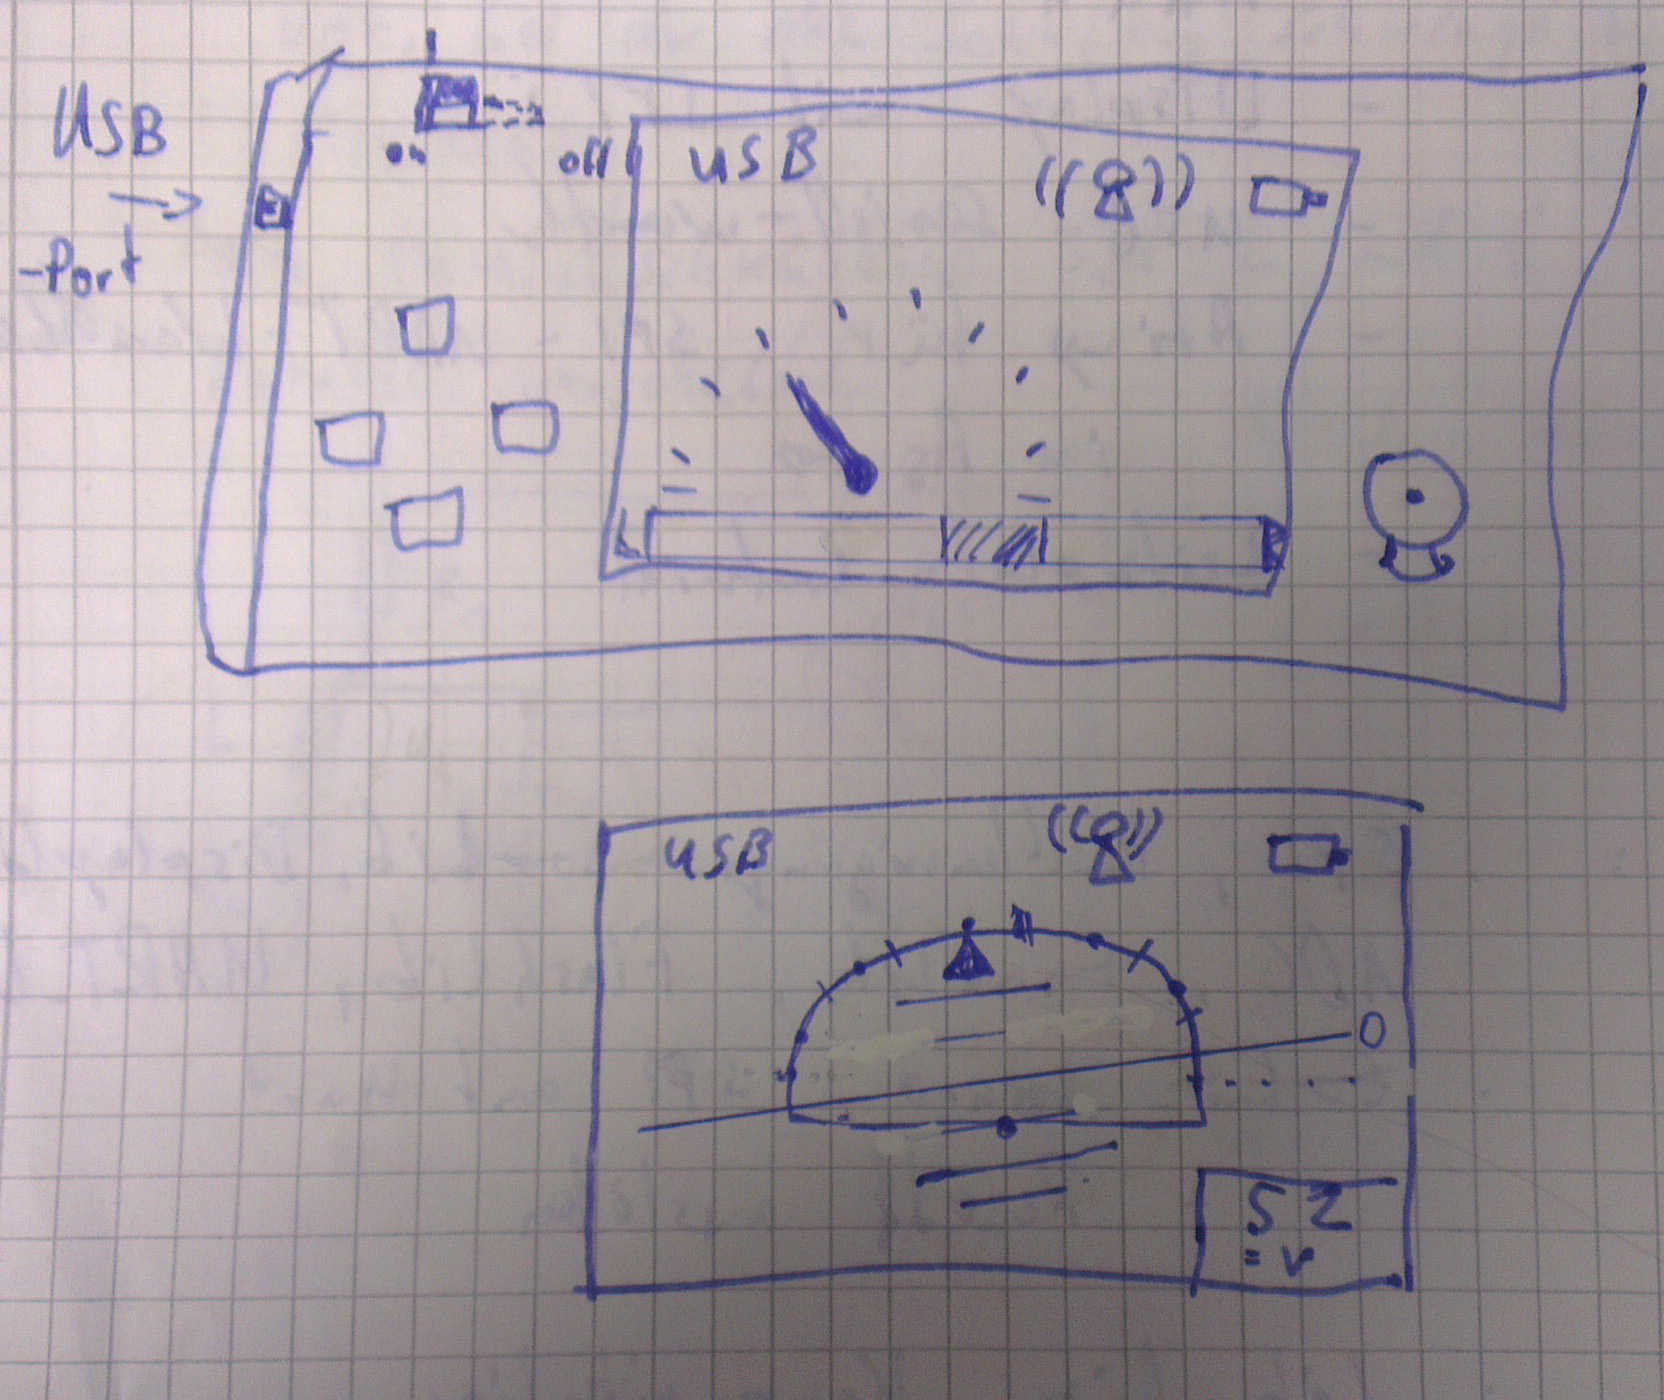
\includegraphics[width=0.7\textwidth]{bilder/idee_controller.jpg}
	\caption{Mögliches Aussehen (Brainstorming)}
	\label{img:idee_controller}
\end{figure}


